\documentclass[12pt]{report}
\usepackage[utf8]{inputenc}
\usepackage{graphicx}
\usepackage{float}
\usepackage{pgfgantt}
\usepackage{hyperref}
\usepackage{algorithm2e}
\usepackage[left=2cm,right=2cm,top=2cm,bottom=2cm]{geometry}
\usepackage[backend=biber]{biblatex}
\usepackage[toc]{glossaries}
\usepackage{appendix}
\makeglossaries

\addbibresource{references.bib}

\bibliography{references}

% Comments
\usepackage{color}
\usepackage[normalem]{ulem} %pour le format barré
\newcommand{\hcp}[1]{\textcolor{blue}{[#1]}}
\newcommand{\hcr}[2]{\textcolor{red}{\sout{[#1]} - \textcolor{blue}{ [#2]}}}
\newcommand{\hc}[1]{\textcolor{red}{[#1]}}
\newcommand{\hcc}[1]{\textcolor{green}{Pour info - [#1]}}

\begin{document}
	\begin{titlepage}
		
		\newcommand{\HRule}{\rule{\linewidth}{0.5mm}} % Defines a new command for the horizontal lines, change thickness here
		
		\center 
		\HRule \\[0.4cm]
		{ \huge \bfseries Report \\Representation and relative positioning from visual information}\\[0.4cm]
		\HRule \\[1.5cm]
		
		\begin{minipage}{0.4\textwidth}
			\begin{flushleft} \large
				\emph{Submitted by:}\\
				\textsc{Asma BRAZI}
			\end{flushleft}
		\end{minipage}
		~
		\begin{minipage}{0.4\textwidth}
			\begin{flushright} \large
				\emph{Supervised by:} \\
				\textsc{Cédric HERPSON}\\
			\end{flushright}
		\end{minipage}\\[4cm]
		
		
		{\large Laboratory of Computer Sciences, Paris 6 \\ Sorbonne University - Faculty of Sciences and Engineering}\\[3cm] 
		{\large June - July 2019 }\\[3cm] 
		
\includegraphics[width=0.6\textwidth]{res/logo.png}\\[1cm] 
		\vfill % Fill the rest of the page with whitespace
		
	\end{titlepage}
	\tableofcontents
	\chapter{Abstract}
	\chapter{Introduction}
	\paragraph{}
	The internship at Laboratory of Computer Sciences, Paris 6 (LIP6) was mainly considered as a continuation of works that we carried out during a university project in first Master's degree. These previous works presented a naive approach of object recognition and an exploration strategy that allows an autonomous robot with a camera to roughly reconstruct its environment.
	
	\paragraph{}
	During this internship, we focused the most on the object recognition, because it was the processing which took the most time to execute. To remedy this situation, we rely on a learning approach where the robot becomes able to recognize an object based on its knowledge. Unlike our previous work where the robot was trying to match the detected object in its environment with all objects in the database, hoping to recognize it.
	
	\paragraph{}
	We summarize in this report our work and the results obtained.
	
    \chapter{Reviews of Existing Work}
	
	\paragraph{}
	The main purpose of our works is to improve the functionalities developed previously. These functionalities allowed the autonomous robot to move in its environment and explore it. The visual information brought by the exploration is used to build a virtual 3D representation of this environment, and to recognize a target object. The target object is an object from the knowledge database. It is specified by the user, at the launching of the application.
	
	\paragraph{}
	In short, our previous strategy can be summarized as follows:
	\begin{itemize}
		\item At each move, the autonomous robot took a picture and analyzed it.
		\item The analysis of the picture brought new knowledge to the autonomous robot.
		\item With this new knowledge, The autonomous robot was able to represent its environment and to recognize the target object.
	\end{itemize}

	\paragraph{}
	However, we assumed some hypothesis that facilitated the process of the exploration. For example, we placed some objects in each corner of the environment and every time the autonomous robot met these objects, it concluded that this was a wall end. So the autonomous robot relied on these objects to decide whether or not it finished exploring the current wall. 
	
	\paragraph{}
	To no longer depend on this hypothesis, we present in our works another manner to construct the environment. Firstly, the autonomous robot does not try to detect the walls anymore by detecting corners. Instead, it takes a picture, analyzes it to extract the contours of the environment. With these contours, the robot decides if it is in front of a face, or if it still has a way to go...etc.
	
	By this way, the autonomous robot gathers the analysis's results to estimate the dimensions of the walls.
	
	\paragraph{}
	Regarding the lengths and heights of walls, we globally estimate them in the same way as in the previous works. Nevertheless, the algorithm behind the calculations that we will develop later, is a little bit different. 

    \chapter{Realization}
    \paragraph{}
    We suppose that the robot is situated in a closed environment, and it has been informed about the target object to serach. 
	\section{Exploration strategy}
	 \subsection{3D modeling}
	 \subsection{Indoor navigation}
	\section{3D Object recognition}
	
	\chapter{Testing}
	\chapter{Conclusion, Limitation and Future work}
	\chapter{References}
	\appendix
	\chapter{List of components}
	\section{Thymio II}
	\textbf{Description} 
	\paragraph{}
	Thymio II is a mobile robot dedicated to the education field. It has many sensors for different purposes. These sensors covered:infrared receiver,proximity, 3 axis accelerometer, ground sensors for line following...etc.
	\\ \\
	\textbf{Data sheet} 
	\paragraph{}
	\url{https://www.generationrobots.com/fr/401213-robot-mobile-thymio-2.htmlURL}
	\begin{figure}[H]
		\begin{center}
			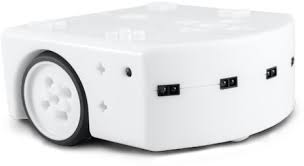
\includegraphics[scale=0.6]{res/thymio.jpg}
		\end{center}
	\end{figure}
	\section{Raspberry-Pi}
	\textbf{Description}
	\paragraph{}
	The Raspberry-Pi is a s single-board computer with wireless LAN and Bluetooth connectivity. It needs a micro USB power supply (2.1 A) in order to be plugged into a power-bank. It has 1GB RAM, 4 USB 2 ports, Full size HDMI, 100 base Ethernet and including a quad core 1.2GHz Broadcom BCM2837 64bit CPU.\\ \\
	\textbf{Data sheet} 
	\paragraph{}
	\url{https://www.raspberrypi.org/products/raspberry-pi-3-model-b/}
	\begin{figure}[H]
		\begin{center}
			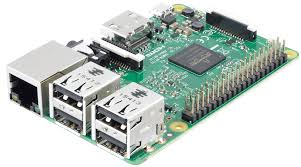
\includegraphics[scale=0.6]{res/raspberry.jpg}
		\end{center}
	\end{figure}
	\section{Raspberry-Pi Camera}
	\textbf{Description}
	\paragraph{}
	The Raspberry-Pi Camera delivers a 5MP resolution image, and 1080p HD video recording at 30 frame/second. It plugs into the Camera Serial Interface connector on the Raspberry-Pi. \\ \\
	\textbf{Data sheet} 
	\paragraph{}
	\url{https://uk.pi-supply.com/products/raspberry-pi-camera-board-v1-3-5mp-1080p?lang=fr}
	\begin{figure}[H]
		\begin{center}
			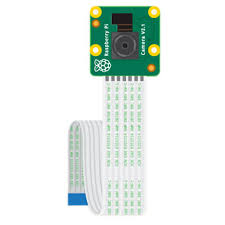
\includegraphics[scale=0.6]{res/camera.jpg}
		\end{center}
	\end{figure}
	\section{Power-bank}
	\textbf{Description}
	\paragraph{}
	For testing, we used RAVPower powerbank to power the Raspberry-Pi. It has 2A input which can charge the 6700 mAh portable charger. this feature guarantees that the Raspberry-Pi's services work correctly. \\ \\
	\textbf{Data sheet} 
	\paragraph{}
	\url{https://www.ravpower.com/p/Ravpower-6700mAh-Portable-Charger.html}
	\begin{figure}[H]
		\begin{center}
			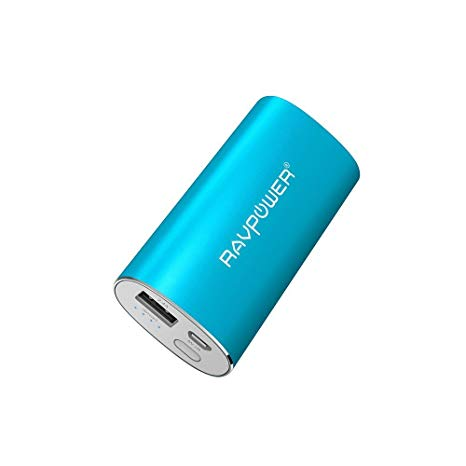
\includegraphics[scale=0.6]{res/power.jpg}
		\end{center}
	\end{figure}
\end{document}